\section{Method}
\label{sec:method}

% \tofix{In order to <enable?/leverage fine-grain sparisty> implement sparse attention for diffusion transformers, we need a mechanism to  (1) (2).. say part 1 and part 2 and describe how that is difficult <challenge>.

% One paragraph to describe the slice figure;}


% Our goal in this work is to: (1) design an efficient sparse attention mechanism that skips query–key dot product computations at a finer granularity, and (2) propose a mechanism for determining a fine-grained attention mask, i.e., identify which slices of attention scores need to be computed or skipped. To this end, we introduce \X, an efficient fine-grained sparse attention mechanism for diffusion transformers. 

\subsection{Overview}
\label{sec:method_attn}
In order to leverage fine-grained sparsity for accelerating the attention layers in diffusion transformers, we must (1) implement a fine-grained sparse attention kernel on modern GPUs that skips computing slices attention scores as shown in Fig.~\ref{fig:method_granularity}, and (2) identify the slices of the attention map (mask) that can be skipped without sacrificing accuracy. To this end, we introduce \X, an efficient fine-grained sparse attention mechanism for diffusion transformers. To implement \X, we propose two techniques to determine the attention mask (\cref{sec:method_maskdetermination}) that determines which attention score slices are to be skipped. This mask is then supplied to \X's sparse attention kernel as input to efficiently compute attention. 
% is then supplied to the \X's sparse attention kernel.  



% Fig.~\ref{fig:method_granularity} shows a section of the attention map of the Wan 1.3B model~\cite{wan}. 
% When computing the attention map, we skip computing qk-dot products that produce $M\times 1$ sections of the attention map for a group of $M$ queries. We skip this computation \emph{only} when we know that \emph{all} attention coefficients is going to be insignificant.

% Fig.~\ref{fig:method_granularity} shows a section of the attention map of the Wan 1.3B model~\cite{wan}. Each row represents the attention scores produced by 256 queries over 128 keys (thus, the figure shows $256\times128$ attention scores). The output token for each query is computed as a weighted sum of the value tokens, the weights being these attention scores. We observe that most query–key pairs yield very small attention scores, with only a few significant outliers. The non-zero scores, which capture correlations between query and key tokens, are distributed irregularly across the map.
\begin{figure}[!htb]
    \centering
    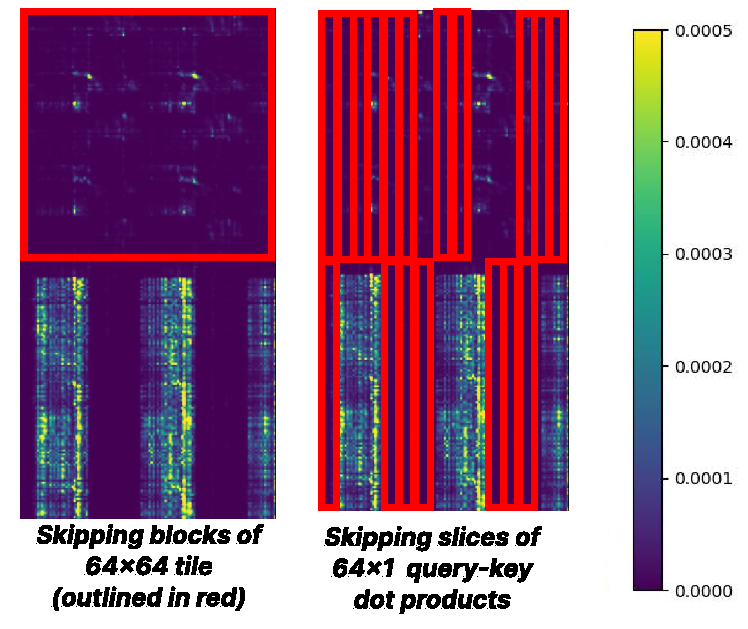
\includegraphics[width=0.65\linewidth]{figs2/fig5.pdf}
    \caption{Block sparse attention mechanisms skip tiles of $128\times128$ attention map scores. We propose a method to skip fine-grain $128\times1$ sections of the attention scores.}
    \label{fig:method_granularity}
\end{figure}


% Current block-sparse attention mechanisms, such as FlexAttention~\cite{flexattn}, BlockSparseAttention~\cite{bsa}, FlashInfer~\cite{flashinfer}, and FlashDecode~\cite{flashdecode}, skip the loading and computation of attention scores over sets of $M$ queries and $M$ keys. In contrast, skipping finer-grained slices of $M$ queries for each key, as illustrated in Fig.\ref{fig:method_granularity}, provides greater opportunities to reduce computation. \X leverages this by skipping $M \times 1$ slices of the attention map.

% Guided by this mask, our \X kernel selectively computes only the required attention scores, as detailed in~\cref{sec:method_acceleratorimplementation}. To compute the sparse attention mask that determines the set of score slices to compute, we propose two training-free strategies for constructing the sparse mask in~\cref{sec:method_maskdetermination}. Finally, we integrate our sparse attention kernel into the video diffusion transformer and evaluate its performance.


\subsection{Representing the Fine-grain Attention Mask}
\label{sec:method_finegrainmask}

% \noindent \textbf{Mask Representation: Sparse-Index Mask.} 
% To mark the set of key/value tokens to be loaded for a group of queries, we use a sequence of integers corresponding to the set of key/value vectors in the HBM that we call the sparse-index mask. At each attention head for a group of $M$ queries, we store an array of integers that correspond to indices of keys/values. For $B$ batches, $H$ heads, $N/M$ groups of queries and at-most $N$ keys, we store these indices as a 4D integer array of dimension $[B, H, N/M, N]$ in memory. $M$ is chosen to be aligned to the accelerator's matrix multiplication hardware's (tensor core's) unit dimension, typically $64/128$ in modern GPUs ($128$ in our implementation in Hopper GPUs). The sparse index mask adds additional memory the same order of magnitude of memory occupied by the tokens. A more detailed overhead analysis is presented in~\cref{sec:method_overheads}. 
% The mask is used to mark the set of key/value tokens to be loaded for a group of $M$ queries at each attention head for our sparse attention kernel. 

To implement fine-grained sparse attention, we need the attention mask to specify which slices of attention map scores to compute, i.e., the key/value vectors required for every group of $M$ queries.
For each group of $M$ queries, we use a sequence of integers corresponding to the key/value vectors in the HBM. This sequence of indices is maintained in an array of integers representing the indices of keys/values to be loaded for each query group, for each attention head. Thus, for $B$ batches, $H$ heads, $N/M$ groups of queries, and up to $N$ keys, these indices are stored as a 4D integer array with dimensions $[B, H, N/M, N]$ in memory. $M$ is selected to align with the unit dimension of the accelerator’s matrix multiplication hardware (tensor cores), typically $64$ or $128$ in modern GPUs (with $128$ used in our implementation on Hopper GPUs). 

% Note that The sparse-index mask introduces additional memory overhead, on the same order of magnitude as the memory occupied by the tokens themselves. A more detailed analysis of this overhead is provided in~\cref{sec:method_overheads}.

% Note that the same set of indices is used to indicate the set of value vectors to be loaded. 

% In addition to storing the set of key/value indices for each group of $M$ queries, we also store a "numindices" array for each attention head that holds the number of indices of key/value tokens to be loaded for a group of $M$ queries.  


\begin{figure*}
    \centering
    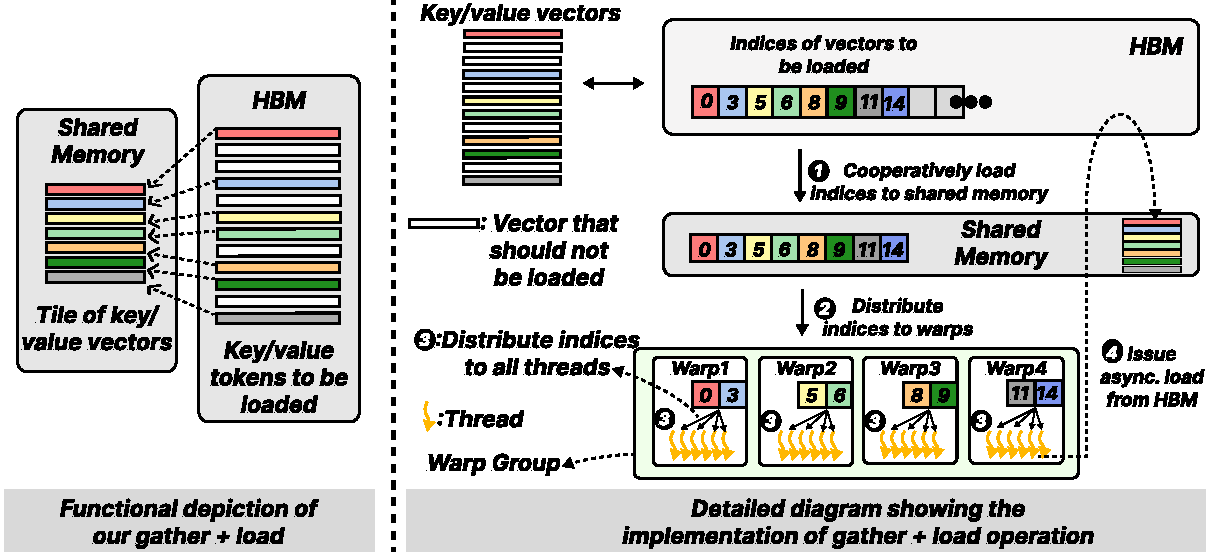
\includegraphics[width=0.85\linewidth]{figs2/fig9_redone.pdf}
    \caption{Loading a sparse set of keys/values using the sparse index mask into a tile in shared memory.}
    \label{fig:method_gatherload}       
\end{figure*}

\subsection{Efficient GPU Kernel Implementation}
\label{sec:method_acceleratorimplementation}

In FlashAttention~\cite{flashattn}, a set of $M$ queries $\mathbf{Q}_{tile}$ and $M$ contiguous keys $\mathbf{K}_{tile}$ are loaded into scratchpad memory before computing $\mathbf{Q}_{tile}\mathbf{K}_{tile}^T$ using the tensor core. On GPUs, these loads are efficiently handled by the Tensor Memory Accelerator (TMA). 
For \X, to compute query-key dot products over a sparse set of keys, we must instead \emph{gather} a set of $M$ non-contiguous keys (identified by the sparse-index mask) and pack them into a tile in on-chip memory. We denote this relevant set of keys for a group of queries as $\mathbf{K}_{rel}$. The query tile and $\mathbf{K}_{rel}$ are then supplied to the tensor core to compute pairwise query-key dot products (i.e, $\mathbf{Q}_{tile}\mathbf{K}_{rel}$).


Loading a sparse set of key/value vectors from memory involves first generating (i.e, computing) the addresses of vector elements belonging to the vectors identified by the  sparse index mask before issuing the load.
To implement our attention mechanism efficiently on GPUs, we must ensure that (i) address generation for loading sparse key/value vectors corresponding to indices in the sparse index mask is fast, and (ii) the latency of address generation is hidden from the critical path to reduce overhead.

To achieve (i), we parallelize address generation by distributing the row indices used for deriving addresses across threads of a warp group. For (ii), we pipeline the address generation routine between loading a tile of key/value vectors and performing attention computation.



\noindent \textbf{Parallelizing address generation with the sparse gather-load primitive.} Given an array of vector indices, the gather-load primitive fetches the corresponding keys from HBM and assembles them in scratchpad as a contiguous tile.
We incorporate this functionality as a device function, called the \emph{gather-load} primitive.
Fig.~\ref{fig:method_gatherload} (left) illustrates its functionality. For each group of $M$ queries, we use the sparse-mask indices to load only the relevant keys onto the chip. 


Figure~\ref{fig:method_gatherload} (right) shows an implementation overview of the gather-load primitive on H100 GPUs. The indices of the key/value vectors, stored in HBM, are provided as input to the sparse attention function. A set of these indices is cooperatively loaded into shared memory~\circled{1}, then distributed across the warps of each warp group (four warps per group on H100)~\circled{2}. Each warp’s index set is then broadcast to all its threads using warp-shuffle instructions~\circled{3}. Finally, based on these row indices, each thread computes the addresses of its assigned vector elements and issues asynchronous load instructions to fetch the sparse vectors into shared memory~\circled{4}.

% Fig.~\ref{fig:method_gatherload} (right) shows an implementation overview of the gather-load primitive function on Hopper H100 GPUs. The indices of the key/value vectors are supplied as input to our sparse attention function and are stored in HBM. A subset of this vector of indices are cooperatively loaded into shared memory~\circled{1}. These indices are then loaded to and distributed across warps of each warp group (set of 4 warps in an H100 GPU)~\circled{2}. The set of all indices to be loaded by each warp is broadcast to all threads~\circled{3}. The broadcast is done using using warp-shuffle instructions. Then, using these row indices, individual addresses of the elements vectors to be loaded by each thread are computed and an asynchronous load instruction to fetch the sparse set of vectors to shared memory~\circled{4}. 
% A detailed implementation snippet is given in the appendix section.


\textbf{Overlap the address generation latency with attention computation.}
The latency of generating addresses for key/value vectors from the sparse index mask can be hidden behind attention computation. On NVIDIA H100 GPUs, the division of work of loading data and performing computation is organized between different warp groups: \emph{producer} warp groups handle data loading, while the \emph{consumer} warp group performs the computation. The producer warp group threads load tiles of query, key, and value vectors into on-chip memory, and the consumer warp group threads compute and accumulate the partial sums of output vectors. %(see~\cref{sec:background_attn}).

An overview of the pipelining strategy is shown in Fig.~\ref{fig:method_pipelining}. In each thread block, a $M$ contiguous query vectors are first loaded into the scratchpad. Loading the relevant keys and values corresponding to these $M$ queries is then performed across many iterations. address generation routine using the \emph{gather-load} primitive function is then invoked (\circled{1}, \circled{2} and \circled{3}). The producer threads load a set of indices corresponding to these $M$ queries from the sparse index mask into shared memory~\circled{1}. 
Following this, the indices are loaded into registers~\circled{2}. These indices correspond to the rows of keys and values that need to be fetched. The producer then issues an asynchronous load operation to retrieve the corresponding rows from global memory~\circled{3}. 
The latency of the asynchronous load is fully hidden by the consumer warp’s computation (attention score and output calculations)~\circled{4}. As a result, our implementation hides latency overhead due to address generation from indirect indices for loading the relevant keys/values into memory.


% Only the keys and values corresponding to indices in the sparse index mask should be loaded from HBM, and this must be done efficiently. This requires an indirect memory access: the program must first load the set of key/value token indices into shared memory, and then load the corresponding tokens themselves. 
\begin{figure}[!htb]
    \centering
    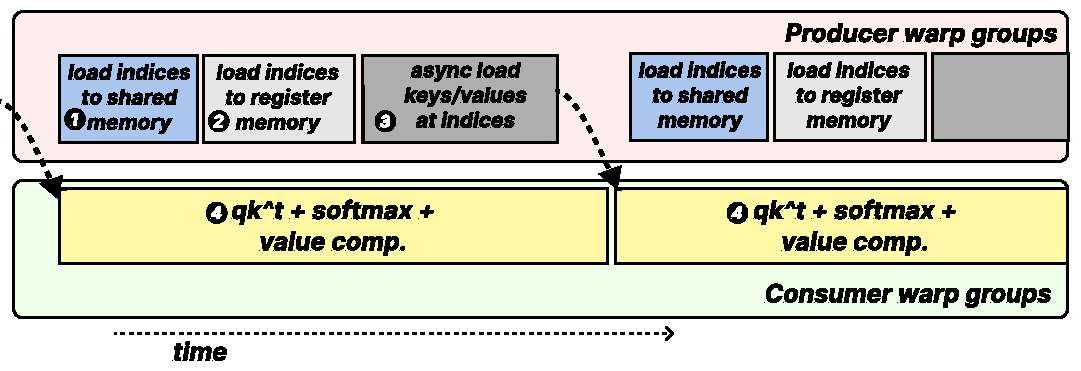
\includegraphics[width=\linewidth]{figs2/fig8.pdf}
    \caption{Pipelining gather-loading of keys/values into shared memory in the producer threads. The sparse index mask indices are loaded into registers first, followed by loading key/value tokens by the producer threads (\emph{gather-load} primitive). The load latency of address generation is hidden by the attention computation.}
    \label{fig:method_pipelining}
\end{figure}



\textbf{End-to-end Implementation overview.}
An overview of our implementation is shown in Fig.~\ref{fig:method_implementationverview}. We build on FlashAttention~\cite{flashattn}, where each thread block computes a unique set of output vectors (shaded red among ``Output Tokens'' in Fig.~\ref{fig:method_implementationverview}). In each thread block, the producer warp groups first load $M$ queries (typically 64 or 128) into scratchpad memory~\circled{1}. In the original FlashAttention~\cite{flashattn} kernel, the producer warp groups then load contiguous blocks of $M$ keys and compute attention scores as described in~\cref{sec:background_attnimpl}.

To implement \X, we modify this design by replacing the full key blocks with slices of $M$ keys, determined by the sparse index mask and fetched using our gather-load primitive~\circled{2}. These sparse key tiles are supplied to the tensor core~\circled{3} to compute only the relevant attention scores. The corresponding value vectors are loaded using the same sparse indices~\circled{4}, and a tensor core operation computes the linear combination of attention scores and value vectors to produce partial output sums~\circled{5}. These partial sums are accumulated into the output vectors~\circled{6}.

The process then advances to the next $M$ slices of keys and values specified by the sparse index mask, and repeats until all relevant indices have been processed~\circled{7}. Across iterations, sparse key/value loading and tensor-core computation are pipelined.


\begin{figure}[!htb]
    \centering
    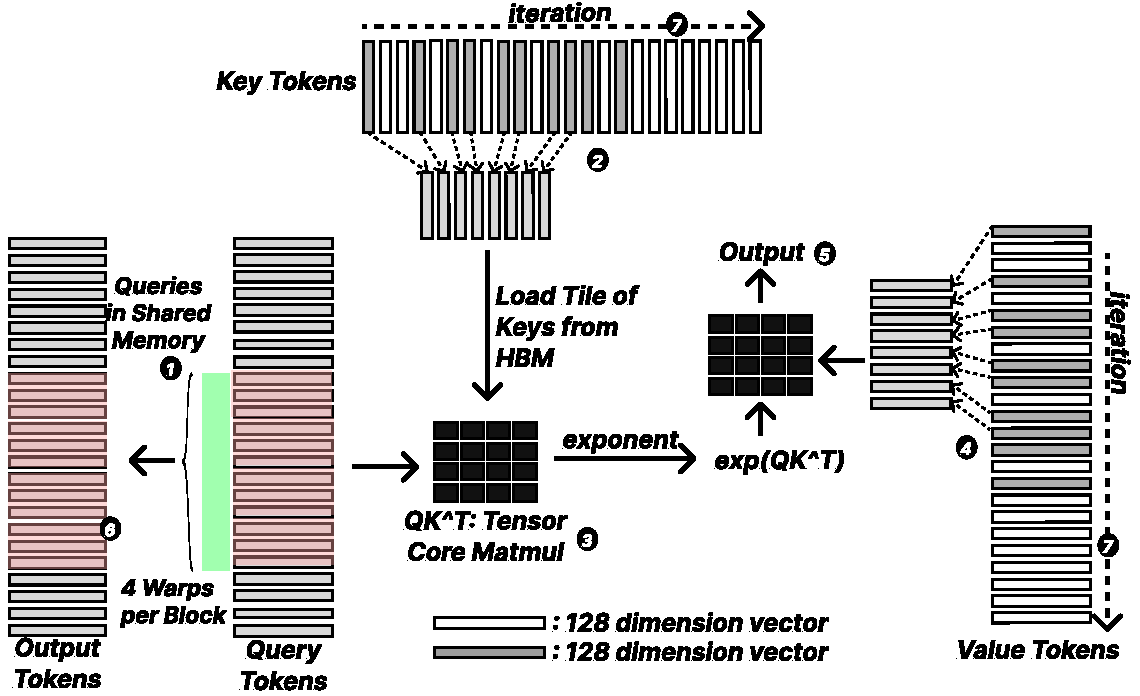
\includegraphics[width=\linewidth]{figs2/fig10}
    \caption{Implementation Overview. At each iteration, a sparse set of keys and values is loaded into the scratchpad. The load operation arranges the relevant keys into a tile in shared memory and uses tensor core operations to compute a partial sum of the output vector. The indices of keys and values to be loaded are supplied by the sparse index mask.}
    \label{fig:method_implementationverview}
\end{figure}



\subsection{Determining the Sparse-Index Mask}
\label{sec:method_maskdetermination}

For a group of $M$ queries $q_1, q_2, \dots, q_M$, we determine whether a key $k$ produces a \emph{significant} attention coefficient with any of them. In this section, we present two training-free strategies for constructing the sparse attention mask.


\textbf{Thresholding by caching attention mask across denoising iterations.}
Prior works~\cite{freecache, d_kv} have observed that across denoising iterations, the intermediate embedding vectors remain approximately unchanged. Leveraging this observation, we cache the sparse index mask derived from significant attention scores in an earlier iteration and reuse it in subsequent ones. Fig.~\ref{fig:maskdeterminationcached} illustrates this approach. At denoising timestep $t$, the sparse attention mask for each attention head is derived from the attention scores that exceeded a predefined threshold in the preceding iteration $(t-1)$.
\begin{figure}[!htb]
    \centering
    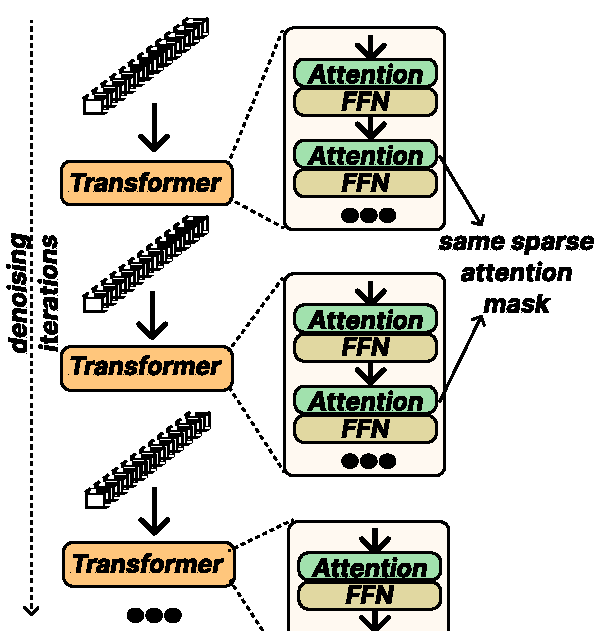
\includegraphics[width=0.7\linewidth]{figs2/fig7.pdf}
    \caption{Determining which slices to attention mask based on attention scores observed in the previous denoising iteration.}
    \label{fig:maskdeterminationcached}
\end{figure}
In practice, we compute the sparse attention mask by evaluating the full attention scores and identifying slices with at least one score above a threshold $\tau_{cached}$. The resulting mask is then stored in HBM for each attention head. In subsequent denoising iterations, this cached mask is reused by our sparse attention mechanism.



\textbf{Thresholding based on average-query.}
In the context of video diffusion models, $q_1, q_2, \dots, q_M$ are query tokens corresponding to adjacent pixels in space and time. Such adjacent tokens typically exhibit similar responses compared to their surrounding queries.
Motivated by this observation, we propose a simple, lightweight strategy for determining the attention mask. We compute the average of a group of queries,
\[
q_{avg}=(q_1+q_2+..+q_M)/M
\]
A key $k$ is included if its dot product with $q_{\text{avg}}$ is significant. We then apply a threshold over these averaged scores. Specifically, the threshold $\tau$ is computed as:
    \[
        \frac{\text{exp}(k.q_{avg}/\sqrt{D})}{D} < \tau_1
    \]

\subsection{Overheads}
\label{sec:method_overheads}
The sparse-index mask adds an additional $O(BHN^2/M)$ to the model’s memory footprint. During attention computation, the producer warp groups load indices from the sparse-index mask onto the chip. This introduces a memory overhead, since the mask must reside in HBM. However, the latency of loading these indices can be hidden from the critical path, resulting in negligible runtime overhead. 

% The latency vs. runtime of the attention scores is shown in Fig
% \tofix{The memory does become significant for the caching technique. I didn't compute the memory footprint yet, I need to do that.}


